% This file is generated by the build script.
\documentclass[10pt,oneside]{book}

\usepackage[a4paper,margin=2.4cm,top=2.5cm,bottom=2.7cm]{geometry}
\usepackage[T1]{fontenc}
\usepackage[utf8]{inputenc}
\usepackage{lmodern}
\usepackage{microtype}
\usepackage{amsmath,amssymb,mathtools}
\usepackage{graphicx}
% Width and height are upper bounds for teaching diagrams, not stretch targets.
\setkeys{Gin}{keepaspectratio}
\usepackage{xcolor}
\usepackage{tcolorbox}
\usepackage{enumitem}
\usepackage{booktabs}
\usepackage{longtable}
\usepackage{tabularx}
\usepackage{caption}
\usepackage{titlesec}
\usepackage{fancyhdr}
\usepackage{hyperref}
\usepackage{bookmark}
\usepackage[section]{placeins}
\usepackage{float}

\tcbuselibrary{skins,breakable}

\providecommand{\tightlist}{%
  \setlength{\itemsep}{0pt}%
  \setlength{\parskip}{0pt}%
}

\providecommand{\pandocbounded}[1]{#1}

% Pandoc marks captionless longtables with \LTcaptype{none}. The 2025
% longtable release expects that value to name a counter, so provide a harmless one.
\newcounter{none}

\definecolor{oxfordblue}{HTML}{002147}
\definecolor{parchment}{HTML}{F8F5EE}
\definecolor{goldaccent}{HTML}{C9A227}
\definecolor{teal}{HTML}{0F766E}
\definecolor{inkgrey}{HTML}{4A4A4A}
\definecolor{paperwhite}{HTML}{FFFFFF}

\hypersetup{
  colorlinks=true,
  linkcolor=oxfordblue,
  urlcolor=oxfordblue,
  citecolor=oxfordblue,
  pdftitle={__BOOK_TITLE__},
  pdfauthor={__BOOK_AUTHOR__},
  pdfsubject={__BOOK_SUBJECT__},
  pdfkeywords={__BOOK_KEYWORDS__}
}

\title{\Huge __BOOK_TITLE__ \\[0.8em] \Large __BOOK_SUBTITLE__}
\author{__BOOK_AUTHOR__}
\date{__BOOK_DATE__}

\newtcolorbox{intuitionbox}{
  enhanced,
  breakable,
  colback=parchment,
  colframe=oxfordblue,
  boxrule=0.8pt,
  arc=1.2mm,
  left=4mm,
  right=4mm,
  top=3mm,
  bottom=3mm,
  title={Intuition},
  fonttitle=\bfseries\color{paperwhite},
  colbacktitle=oxfordblue
}

\newtcolorbox{blackboardbox}{
  enhanced,
  breakable,
  colback=paperwhite,
  colframe=inkgrey,
  boxrule=0.8pt,
  arc=1.2mm,
  left=4mm,
  right=4mm,
  top=3mm,
  bottom=3mm,
  title={Alice's notebook},
  fonttitle=\bfseries\color{paperwhite},
  colbacktitle=inkgrey
}

\newtcolorbox{oxfordbox}{
  enhanced,
  breakable,
  colback=parchment,
  colframe=goldaccent,
  boxrule=0.8pt,
  arc=1.2mm,
  left=4mm,
  right=4mm,
  top=3mm,
  bottom=3mm,
  title={A dream of Oxford},
  fonttitle=\bfseries\color{paperwhite},
  colbacktitle=goldaccent
}

\newtcolorbox{trythisbox}{
  enhanced,
  colback=paperwhite,
  colframe=oxfordblue,
  boxrule=0.8pt,
  arc=1.2mm,
  left=4mm,
  right=4mm,
  top=3mm,
  bottom=3mm,
  title={Try this at home},
  fonttitle=\bfseries\color{paperwhite},
  colbacktitle=oxfordblue
}

\newtcolorbox{prooflightbox}{
  enhanced,
  breakable,
  colback=parchment,
  colframe=inkgrey,
  boxrule=0.8pt,
  arc=1.2mm,
  left=4mm,
  right=4mm,
  top=3mm,
  bottom=3mm,
  title={A gentle proof},
  fonttitle=\bfseries\color{paperwhite},
  colbacktitle=inkgrey
}

\newtcolorbox{hintbox}{
  enhanced,
  breakable,
  colback=parchment,
  colframe=teal,
  boxrule=0.8pt,
  arc=1.2mm,
  left=4mm,
  right=4mm,
  top=3mm,
  bottom=3mm,
  title={Hint},
  fonttitle=\bfseries\color{paperwhite},
  colbacktitle=teal
}

\newtcolorbox{answerbox}{
  enhanced,
  breakable,
  colback=paperwhite,
  colframe=goldaccent,
  boxrule=0.8pt,
  arc=1.2mm,
  left=4mm,
  right=4mm,
  top=3mm,
  bottom=3mm,
  title={Answer},
  fonttitle=\bfseries\color{paperwhite},
  colbacktitle=goldaccent
}

\newtcolorbox{demobox}[3]{
  enhanced,
  breakable,
  colback=parchment,
  colframe=oxfordblue,
  boxrule=0.8pt,
  arc=1.2mm,
  left=4mm,
  right=4mm,
  top=3mm,
  bottom=3mm,
  title={Interactive demo: #1},
  fonttitle=\bfseries\color{paperwhite},
  colbacktitle=oxfordblue,
  before upper={%
    \begin{minipage}{.18\linewidth}
      \includegraphics[width=\linewidth,keepaspectratio]{#3}
    \end{minipage}\hfill
    \begin{minipage}{.77\linewidth}
      \raggedright\small\url{#2}
    \end{minipage}\par\vspace{.35em}%
  }
}

\newcommand{\demourl}[1]{\texttt{#1}}

\begin{document}

\frontmatter
\hypersetup{pageanchor=false}
\maketitle

\begin{center}
\vspace{2em}
\includegraphics[width=0.9\textwidth]{assets/images/cover.pdf}
\vspace{2em}
\end{center}

\clearpage
\hypersetup{pageanchor=true}
\tableofcontents

\chapter{Before you fall}
This book is written for readers who know some high-school mathematics and are curious about the ideas behind multilinear algebra.

Alice will open twelve mathematical rooms. In each one, she first plays with something concrete: arrows, keys, cards, balances, tickets, and maps. Only after the idea has become familiar do we write its formal name.

The main journey uses real scalars and finite-dimensional vector spaces. Marked notes introduce complex scalars and explain which measuring rules change. A superscript used as a component index is a label, not a power. Explicit sums introduce each indexed formula before a shorter notation is used.

The illustrations use the same examples as the calculations beside them. Follow Alice's experiments, compare the pictures with her arithmetic, and then try the exercises. The final room introduces derivatives as local change and integrals as accumulated measurement.

Read the intuition boxes first. They are the doorway. Then read Alice's notebook for the formal rules. Finally, play with the demos on the companion website; they are the playground.

\begin{figure}[htbp]
\centering
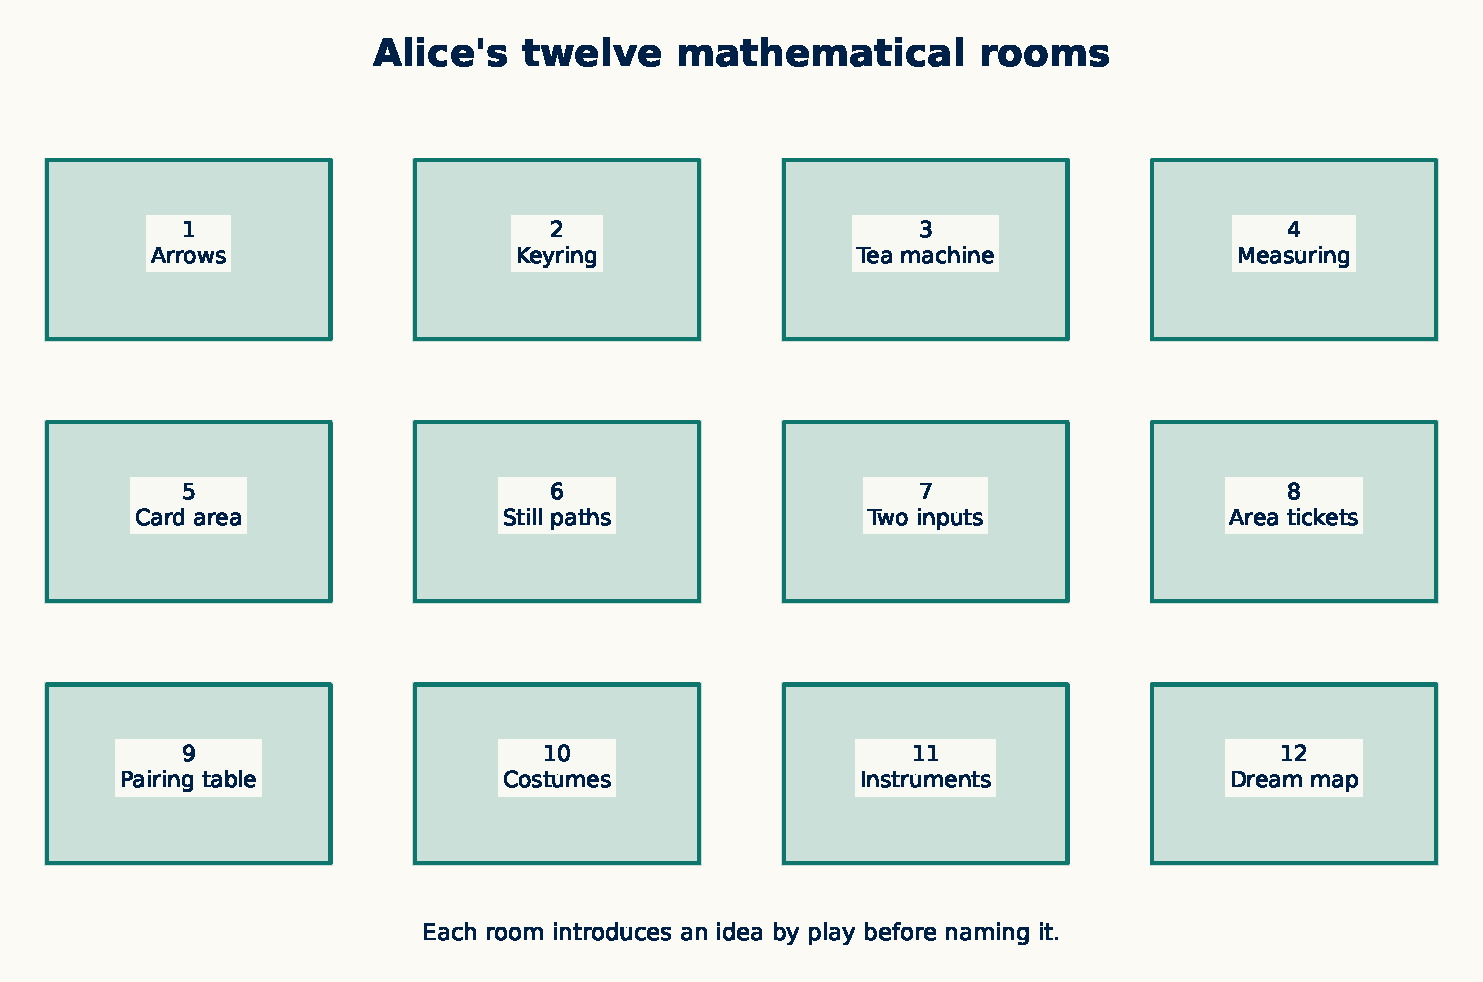
\includegraphics[width=.98\textwidth]{assets/figures/story-map.pdf}
\caption{Alice’s twelve mathematical rooms.}
\end{figure}

\mainmatter
__CHAPTER_INPUTS__

\backmatter
\setcounter{secnumdepth}{0}
\addtocontents{toc}{\protect\setcounter{tocdepth}{1}}
\input{backmatter/answers.tex}

\chapter{Glossary}
\textbf{Scalar.} A number from a specified field, here usually $\mathbb R$ and in marked notes $\mathbb C$.

\textbf{Vector.} An element of a vector space. A real Euclidean arrow is a first geometric example; length requires a measuring rule.

\textbf{Basis.} A linearly independent spanning set; every vector has unique scalar coefficients in that basis.

\textbf{Covector.} A linear scalar-valued question on a vector space. Covectors form its dual space.

\textbf{Linear map.} A transformation that preserves addition and scaling.

\textbf{Inner product.} A positive-definite pairing that defines length and orthogonality. Real inner products are symmetric bilinear; complex inner products involve conjugation.

\textbf{Determinant.} A scalar associated with a square matrix that detects invertibility. Over $\mathbb R$, it gives a signed volume factor.

\textbf{Eigenvalue.} A stretching factor associated with a special direction.

\textbf{Bilinear form.} A scalar-valued map linear in each of two vector inputs separately.

\textbf{Tensor.} An element of a tensor-product space; in finite dimensions it can be described by a multilinear map on appropriate vector and covector inputs.

\textbf{Tensor type and order.} Type counts the vector and covector factors; order counts all factors or slots.

\textbf{Tensor rank.} The fewest pure products needed to express a tensor as a sum; zero has rank zero.

\textbf{Wedge product.} An alternating exterior product. Simple real vector wedges represent oriented patches; their magnitudes require an inner product.

\textbf{Differential form.} A smooth field of alternating covector tensors used to measure oriented regions of the matching dimension.

\textbf{Exterior derivative.} The operator $d$ that takes a smooth $k$-form to a smooth $(k+1)$-form.

\textbf{Traction.} Force per unit area across an oriented surface, given by stress acting on its unit normal.

\chapter{Symbols}
\begin{longtable}{lp{.65\textwidth}}
$\mathbb R,\mathbb C$ & real and complex scalar fields\\
$V,V^*$ & a vector space and its space of linear covectors\\
$\mathbf e_i,\epsilon^i$ & a basis and its dual basis; $i=1,\ldots,n$\\
$\mathbf{v}$ & a vector\\
$\|\mathbf{v}\|$ & the length of $\mathbf{v}$\\
$\langle \mathbf{u},\mathbf{v}\rangle$ & inner product\\
$T$ & a linear map or tensor, as specified in context\\
$A$ & a matrix\\
$\det A$ & determinant of $A$\\
$\lambda$ & an eigenvalue\\
$B(\mathbf{u},\mathbf{v})$ & a bilinear form\\
$\mathbf{u}\wedge\mathbf{v}$ & wedge product\\
$U\otimes V$ & tensor product\\
$v^i\in\mathbb R$ & a vector component in the main real examples\\
$\alpha_i\in\mathbb R$ & a covector component in the main real examples\\
$\delta^i{}_j$ & one if $i=j$, zero otherwise\\
$\alpha_i v^i$ & $\sum_{i=1}^n\alpha_i v^i$, using Einstein summation\\
$\overline z,\lvert z\rvert$ & complex conjugate and complex modulus\\
$\Lambda^k(V)$ & the exterior space of $k$-vectors\\
$T_pU,T_p^*U$ & tangent vectors and covectors at the point $p$\\
$\Omega^k(U)$ & smooth differential $k$-forms on $U$\\
$\omega$ & a differential form\\
$dx,dy$ & coordinate covectors reading tangent components\\
$d\omega$ & the exterior derivative of a form\\
$\partial M$ & the boundary of an oriented region\\
$\sigma,\mathbf n,\mathbf t$ & stress, unit surface normal, and traction\\
$D,\mathbf J,\nabla c$ & diffusion tensor, flux, and concentration gradient\\
$I,\boldsymbol\omega,\mathbf L$ & inertia tensor, angular velocity, and angular momentum\\
$g_{ij}$ & metric coefficients in a chosen coordinate basis\\
\end{longtable}

\chapter{Further reading}
\begin{itemize}
\item Gilbert Strang, \emph{Introduction to Linear Algebra}.
\item Sergei Lang, \emph{Introduction to Linear Algebra}.
\item Michael Spivak, \emph{Calculus on Manifolds}.
\item Loring Tu, \emph{An Introduction to Manifolds}.
\item Theodore Frankel, \emph{The Geometry of Physics}.
\end{itemize}

\chapter{About the demos}
Every chapter has an interactive demo on the companion website.
The QR codes in the demo boxes link directly to the live demos.
The site is:

\begin{center}
\texttt{__BOOK_URL__}
\end{center}

\end{document}
